\documentclass{letter}
\usepackage{wallpaper}
\usepackage{geometry}
\usepackage{xcolor}
\usepackage[T1]{fontenc}
\usepackage[scaled]{helvet}
\usepackage{fontawesome5}
\usepackage{hyperref}
\usepackage[none]{hyphenat}
\usepackage{enumitem}
\usepackage{graphicx}
\usepackage{multicol}
\graphicspath{ {./img/} }

\setitemize{noitemsep, topsep=0.05em, leftmargin=0.2in, itemsep=0.05em}
\setlength{\columnsep}{5cm}

\renewcommand{\familydefault}{\sfdefault}

\geometry{
  paperwidth=\dimexpr\textwidth+\marginparsep+\marginparwidth\relax,
  paperheight=\dimexpr\textheight+\footskip\relax,
  left=20pt,
  right=20pt,
  top=0pt,
  bottom=0pt,
  nohead,
  nofoot,
  nomarginpar
}

\ThisCenterWallPaper{1.5}{./img/cvbg.png}

\begin{document}

\begin{minipage}[t]{0.40\textwidth}
\setlength{\baselineskip}{1.5\baselineskip}
\color{white}
\vspace{1cm}
{\large Personal Information}

\rule{\linewidth}{0.4pt}

\faPhone \quad \input{phone.tex} 
% Check phoneExample.tex

\faEnvelope \quad \href{malfi.bruno@gmail.com}{malfi.bruno@gmail.com}

\faMapMarker \quad Valencia

\rule{\linewidth}{0.4pt}

{\large Links}

\faLinkedin \quad \href{https://www.linkedin.com/in/bruno-malfi-fabeiro}{LinkedIn}

\faGithub \quad \href{https://github.com/BrunoMalfi}{Github}

\faPaperclip \quad \href{https://github.com/BrunoMalfi/CV/blob/main/CV_EN.md}{Extended CV}

\rule{\linewidth}{0.4pt}

{\large Technologies}

\faNodeJs \quad Node.js

\faReact \quad React

\faVuejs \quad Vue

\faAngular \quad Angular

\faLinux \quad Bash

\faCircleNotch \quad XSLT

\rule{\linewidth}{0.4pt}

{\large Languages}

\faLanguage \quad Spanish

\faLanguage \quad English

\faLanguage \quad Italian

\end{minipage}
\hfill
\begin{minipage}[t]{0.60\textwidth}
\setlength{\baselineskip}{1.5\baselineskip}
\vspace{0.8cm}

\begin{minipage}{0.8\linewidth} 
    {\huge Bruno Malfi Fabeiro}

    {\large Programmer}
\end{minipage}
\begin{minipage}{0.1\linewidth}
    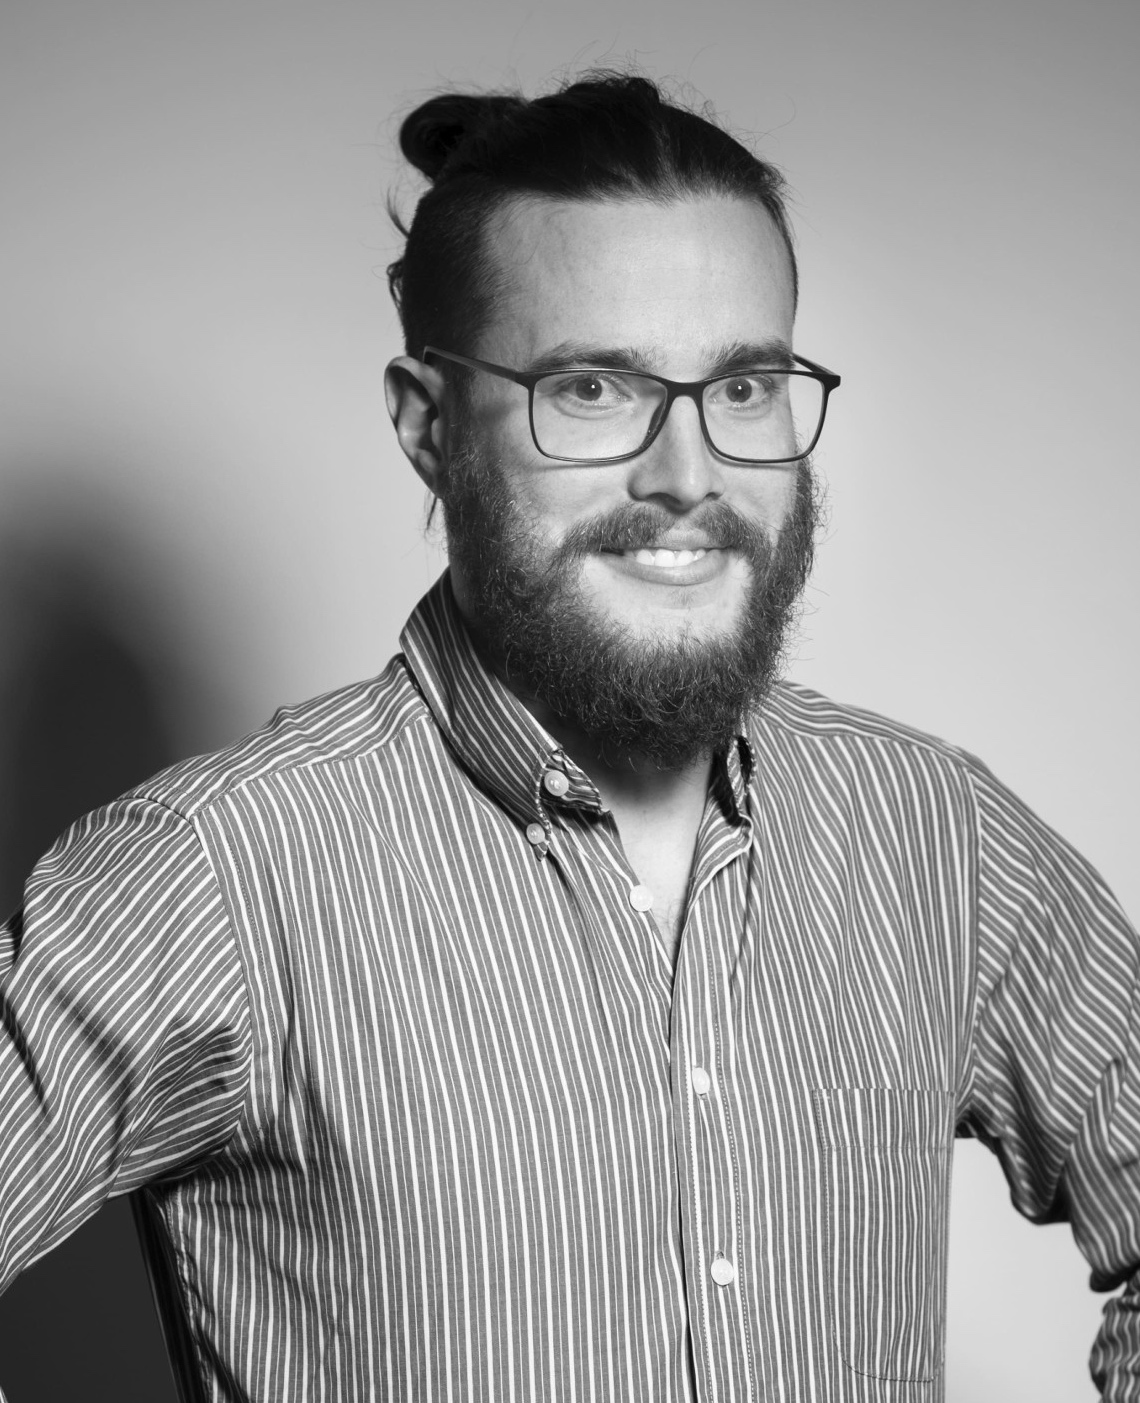
\includegraphics[width=1.5cm, height=2cm]{foto2.jpg}
\end{minipage}

\vspace{0.2cm}
 
9 years of experience in the IT sector.
Technical degree, Engineering, and FullStack Bootcamp.
But, above all, eager for new challenges.

\vspace{0.5cm}

{\large Professional Experience}
\rule{\linewidth}{0.4pt}
{\large \textbf{FullStack Programming}}

{\small MAR 2024 - Present}

\begin{itemize}
    \item Projects in \faHtml5 HTML, \faCss3 CSS, \faJs Vanilla  JavaScript and \faBootstrap Bootstrap
    \item Backend in Node.js using Express, Sequelize, Mongoose, etc.
    \item Frontend, mainly in React but also in Vue and Angular.
\end{itemize}

{\large \textbf{EDI Consultant/Technician, Freelance}}

{\small SEP 2018 - MAR 2024}

\begin{itemize}
    \item EDI Consulting for DWID/Hillside and ETRIS BANK clients. Same tech I worked with in Derwid
\end{itemize}

{\large \textbf{EDI Consultant/Technician at DERWID (Villach, Austria)}}

{\small JUL 2017 – SEP 2018}

\begin{itemize}
    \item EDI Consulting for Derwid clients.
    \item Maps in XSLT. Scripts in Linux Bash.
    \item Configuration of MySQL tables with Workbench or PhpMyAdmin.
\end{itemize}

{\large \textbf{EDI Consultant/Technician at EDICOM (Valencia)}}

{\small MAY 2015 - MAY 2017}
\begin{itemize}
    \item EbiMap maps. JavaScript scripts.
\end{itemize}

{\large Education}
\rule{\linewidth}{0.4pt}

{\large \textbf{FullStack Developer Bootcamp, EDEM (Master)}}

{\small MAR 2024 - JUL 2024}

{\large \textbf{Telecommunications Engineering, UPV (Bachelor's)}}

{\small SEP 2011 - JUN 2015}

\end{minipage}
\end{document}
